\chapter{Results}\label{sec:results}
\lhead{\emph{Results}}

In this section, we will discuss the results found during the experiments. As mentioned in Section \ref{sec:performance_measures}, two performance measures were taken into account. First, we will report the accuracy scores as found by the visualization assay. This will be a measure of how good a dimensionality reduction technique was at portraying the data in two dimensions while preserving most information. Secondly, the time it took to perform these analyses are reported. Here we will evaluate the time-wise computational cost and scalability of NUTS and VB and compare them with each other.

\section{Visualization performance}
We start with the results of the visualization assay. A logistic regression was performed on each latent data-set plot to predict cell-types in the plots, where the accuracy of this result was noted. This was done using a $5$-fold cross-validation scheme. The average accuracy of the five folds was taken as the accuracy of a plot. In the case of the HmPPCAs models, the accuracy was computed for each level. Since the levels contained multiple plots, the accuracy of one level was computed as the weighted average of each plot within that level, where the weights were determined by the number of data-points that were contained within each plot. When the overall accuracies of HmPPCAs models are reported, the accuracy of the best performing level is given.

% \begin{wrapfigure}{l}{0.35\textwidth}
%   \begin{center}
%     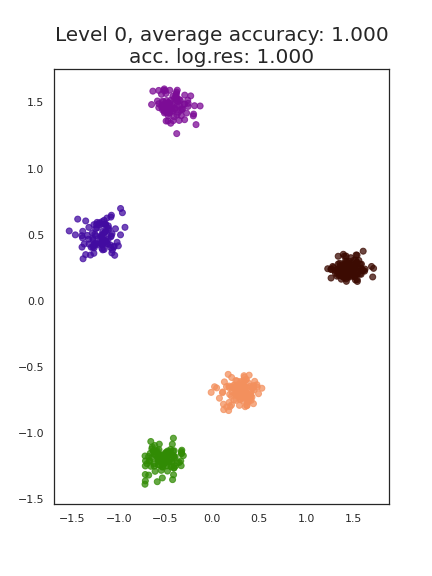
\includegraphics[width=0.35\textwidth]{figs/simple_5_nuts.png}
%   \end{center}
%   \caption{Birds}
% \end{wrapfigure}

% \begin{wrapfigure}{r}{0.35\textwidth}
%   \begin{center}
%     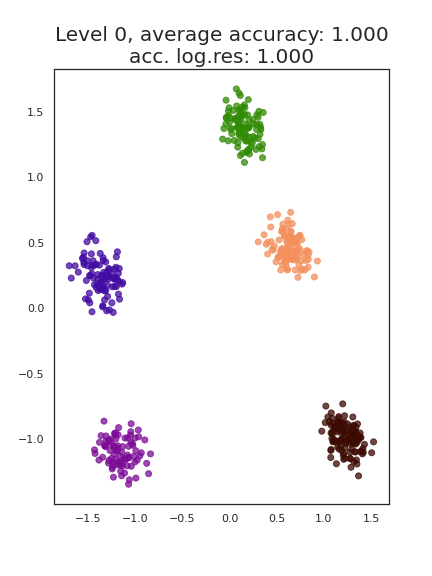
\includegraphics[width=0.35\textwidth]{figs/simple_5_vb.png}
%   \end{center}
%   \caption{Birds}
% \end{wrapfigure}

\begin{table}
\setlength{\tabcolsep}{3pt}
\caption[Accuracy of multinomial logistic regressions on the latent data-sets found by each model in a $5$-fold cross-validation scheme.]{\textbf{Accuracy of multinomial logistic regressions on the latent data-sets found by each model in a $5$-fold cross-validation scheme. The highest accuracy for a particular data-set is indicated in bold.}}
    \label{tab:results}
    \centering
    \small
    \begin{tabular}{l|rrrrr|rrrrr|r|r}
          & \multicolumn{5}{r}{Splatter simple} & \multicolumn{5}{r}{Splatter complex} & Darmanis & Nestorowa \\
          genes & 5 & 25 & 50 & 150 & 250 & 5 & 25 & 50 & 150 & 250 & 500 & 500 \\
          \hline
        
        \makecell{PPCA\\(NUTS)} & \textbf{1.00} & 0.88 & 0.99 & 0.97 & 0.94 &
        0.80 & 0.68 & 0.82 & 0.81 & 0.77 & 0.60 & 0.73\\
        
        \makecell{HmPPCAs\\(NUTS)} & \textbf{1.00} & \textbf{1.00} & \textbf{1.00} & 0.97 & \textbf{1.00} &
        0.90 & 0.82 & 0.89 & 0.82 & 0.77 & 0.70 & 0.79\\
        
        \makecell{PPCA\\(VB)} & \textbf{1.00} & 0.88 & 0.99 & 0.96 & 0.94 &
        0.80 & 0.69 & 0.81 & 0.82 & 0.76 & 0.73 & 0.73\\
        
        \makecell{HmPPCAs\\(VB)} & \textbf{1.00} & \textbf{1.00} & \textbf{1.00} & 0.98 & \textbf{1.00} &
        0.90 & 0.91 & 0.90 & 0.94 & 0.79 & 0.73 & 0.79\\
        
        UMAP & \textbf{1.00} & \textbf{1.00} & \textbf{1.00} & \textbf{1.00} & \textbf{1.00} &
        0.95 & \textbf{0.98} & 0.98 & \textbf{1.00} & \textbf{1.00} & \textbf{0.82} & \textbf{0.82}\\
        
        t-SNE & \textbf{1.00} & \textbf{1.00} & \textbf{1.00} & \textbf{1.00} & \textbf{1.00} & 
        \textbf{0.95} & 0.94 & \textbf{1.00} & \textbf{1.00} & \textbf{1.00} & 0.76 & 0.80\\
    \end{tabular}
    % \medskip
    % \small
    % The table shows the accuracy of a 5-fold cross validation scheme when performing a logistic regression on the latent data. In case of the hmPPCAs models, the weighted average accuracy of all plots on a level was taken and the accuracy on the level with the highest accuracy is shown. For PPCA, PPCA on the top-level of hmPPCAs was used.
\end{table}




\begin{figure}
    \centering
    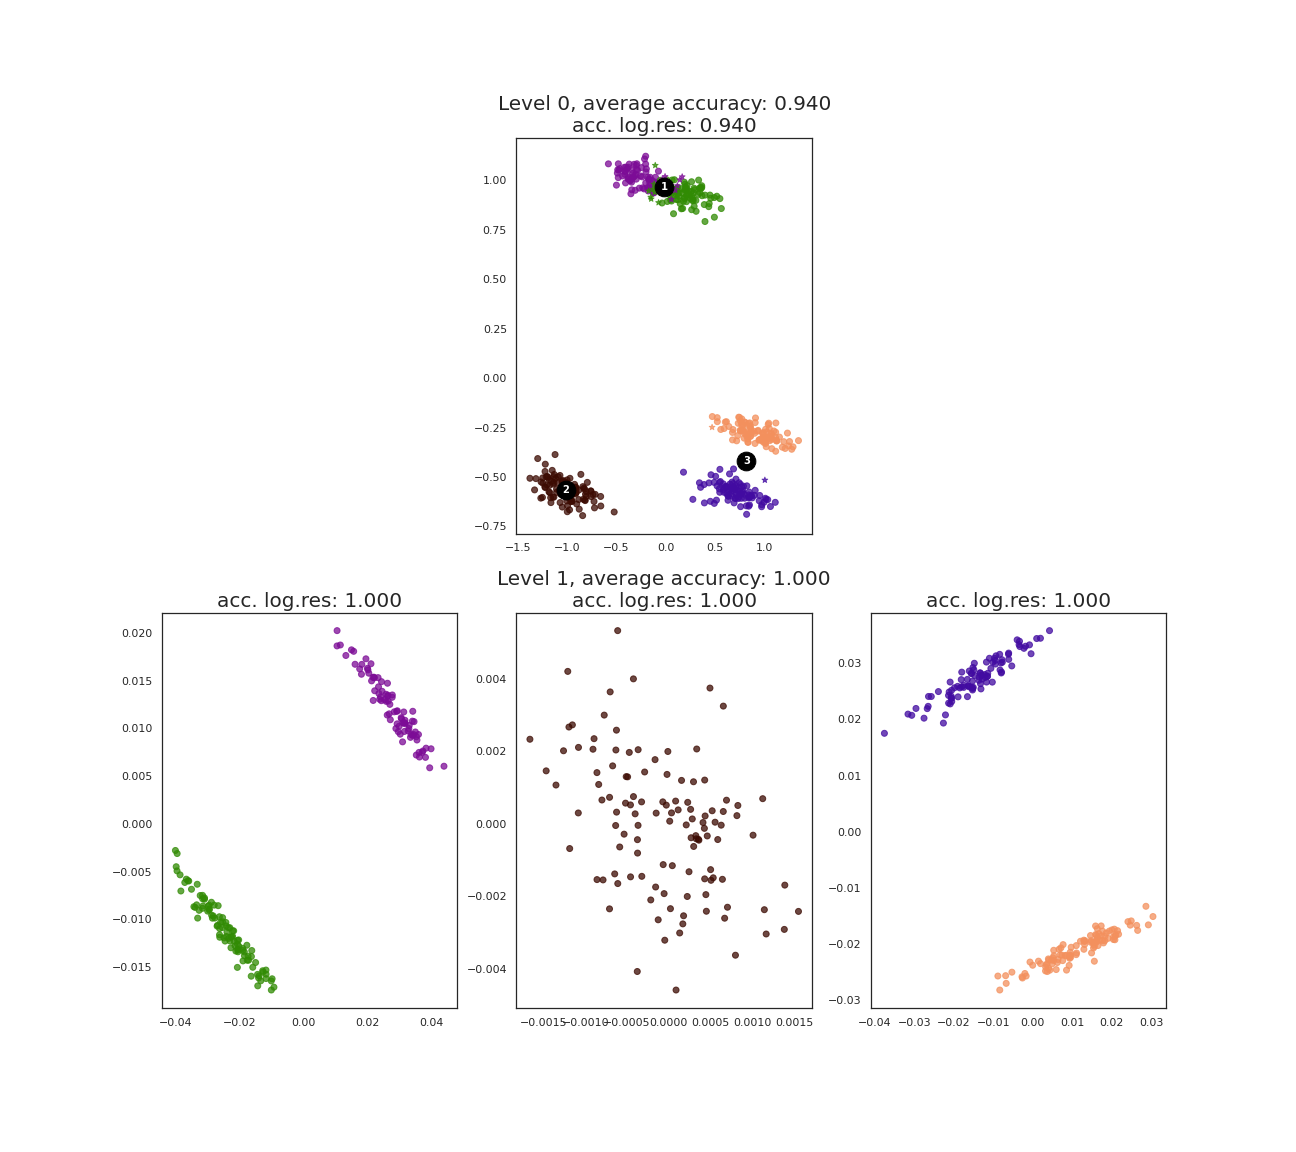
\includegraphics[width=\linewidth]{figs/simple_250_nuts.png}
    \caption[HmPPPCAs model performed on the simple Splatter data-set with 250 genes using NUTS]{\small \textbf{HmPPPCAs model performed on the simple Splatter data-set with 250 genes using NUTS.} \small The maximum accuracy of $1.0$ was found at level $1$. The top-level PPCA achieved an accuracy of $0.940$. The clusters found within the top-level PPCA have been numbered. The colours indicate different cell types. Data-points that were predicted correctly by the logistic regression are plotted with dots, incorrect predictions are plotted with stars.}
    \label{fig:simple_250_nuts}
\end{figure}



\begin{figure}
    \centering
    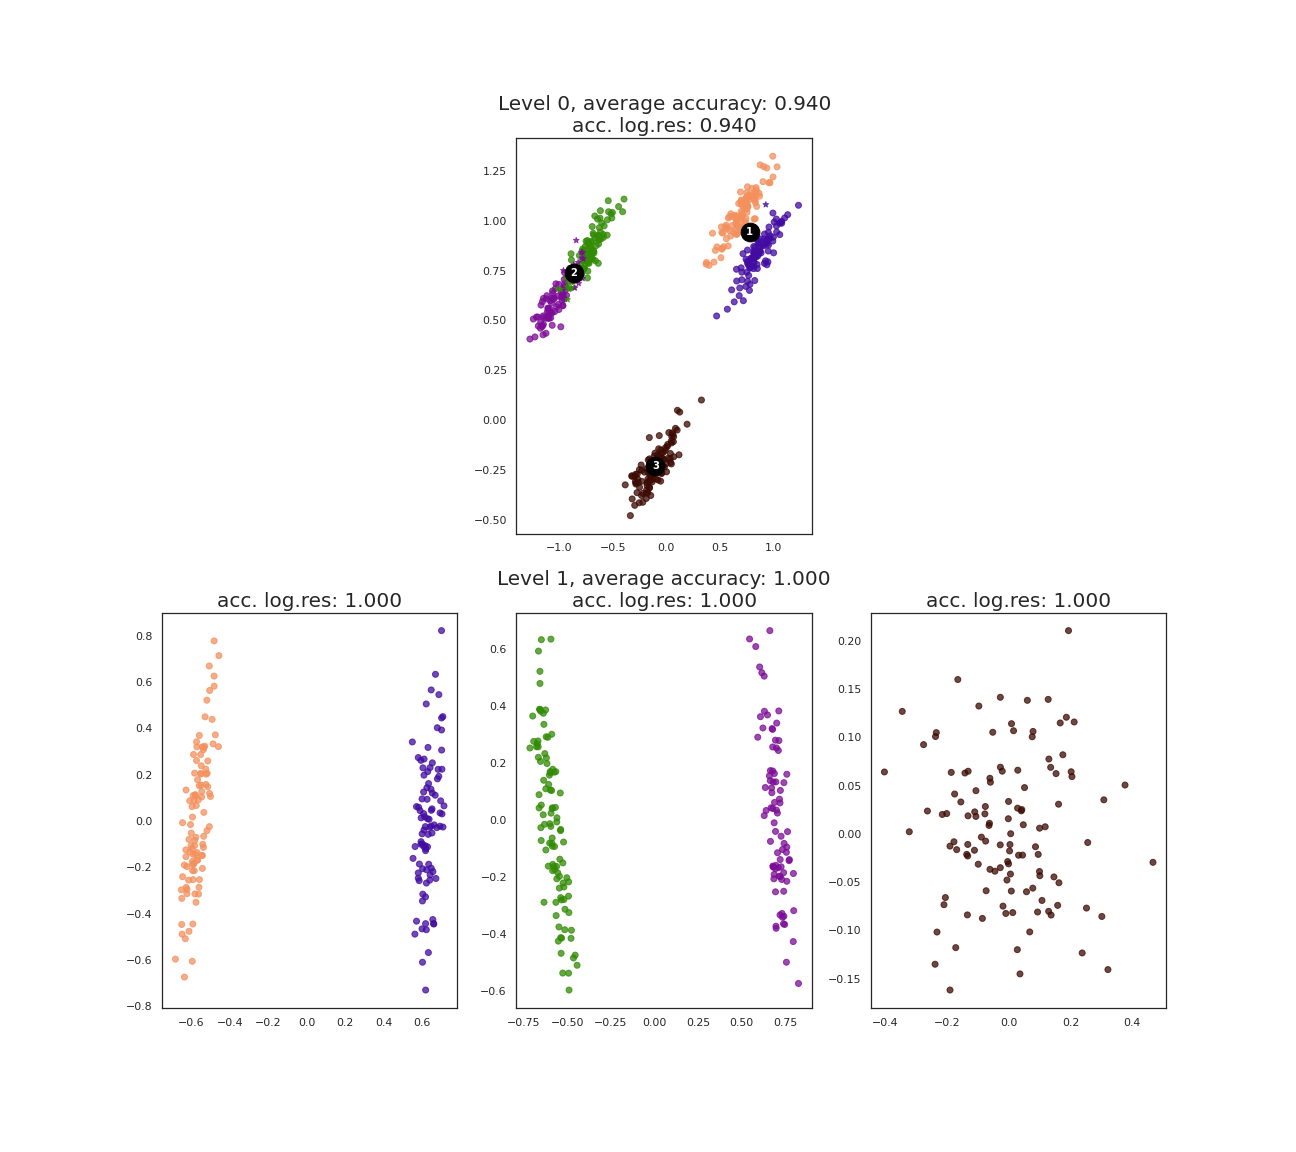
\includegraphics[width=\linewidth]{figs/simple_250_vb.png}
    \caption[HmPPPCAs model performed on the simple Splatter data-set with 250 genes using VB]{\small \textbf{HmPPPCAs model performed on the simple Splatter data-set with 250 genes using VB.} \small The maximum accuracy of $1.0$ was found at level $1$. The top-level PPCA achieved an accuracy of $0.940$. The clusters found within the top-level PPCA have been numbered. The colours indicate different cell types. Data-points that were predicted correctly by the logistic regression are plotted with dots, incorrect predictions are plotted with stars.}
    \label{fig:simple_250_vb}
\end{figure}

All results found are given in Table \ref{tab:results}. The simple Splatter data-sets were converted to their top-level latent spaces first by PPCA. Figure \ref{fig:simple_250_nuts} shows the results on the simple Splatter 250 genes data-set when using NUTS and Figure \ref{fig:simple_250_vb} shows the results when using VB. The figures for the data-sets containing fewer genes are given in Appendix \ref{sec:simple}. We see that reasonable accuracy scores ($>0.88$) were achieved on the visualization assay on the top-level latent data. When more levels of depth were added by use of the HmPPCAs, these accuracy scores almost always rose to $1.0$.

When evaluating the complex Splatter data-sets, lower and more varying accuracies were observed. The results when analysing the 250 genes complex data-set are shown in Figure \ref{fig:complex_250_nuts} (NUTS) and Figure  \ref{fig:complex_250_vb} (VB). The results of the lower dimensional data-sets are given in Appendix \ref{sec:complex}. When comparing PPCA and HmPPCAs, we see that the addition of more levels increased the accuracy in almost every case, although neither was able to achieve perfect accuracy scores on the complex data-sets. When we compare NUTS and VB, we see that their results are very similar when performing the PPCA. Occasionally, the scores of NUTS and VB differed, but the difference was always negligible. In the case of the HmPPCAs, however, larger differences between NUTS and VB were observed. VB performed better than or at least as good as NUTS in all cases when comparing the HmPPCAs results.

Both methods achieved lower scores on the Darmanis and Nestorowa data-sets than on the Splatter data-sets. Figures \ref{fig:damanis_nuts} and \ref{fig:darmanis_vb} show the result of the HmPPCAs on the Darmanis data-set when using NUTS and VB, respectively. Figures \ref{fig:nestorowa_nuts} and \ref{fig:nestorowa_vb} are the NUTS and VB HmPPCAs results when analyzing the Nestorowa data-set. The HSPC cell types in this data-set showed multiple clusters. When using NUTS, the HmPPCAs separated each of those clusters. The progenitor and LT.HSC cells were difficult to distinguish from each other. When using VB, fewer levels were initialized and therefore the data was separated less. Since a higher accuracy was achieved using NUTS on level $2$, it might have been the case that NUTS was able to obtain a slightly better visualization which led to further clustering. Again, HmPPCAs scored higher than PPCA on the Nestorowa data-sets with both NUTS and VB and on the Darmanis data-set when using NUTS. The addition of more levels did not improve the accuracy on the Darmanis data-set when using VB. VB yielded better results than NUTS on the Darmanis data-set, but both methods performed exactly equally on the Nestorowa data-set.



\begin{figure}
    \centering
    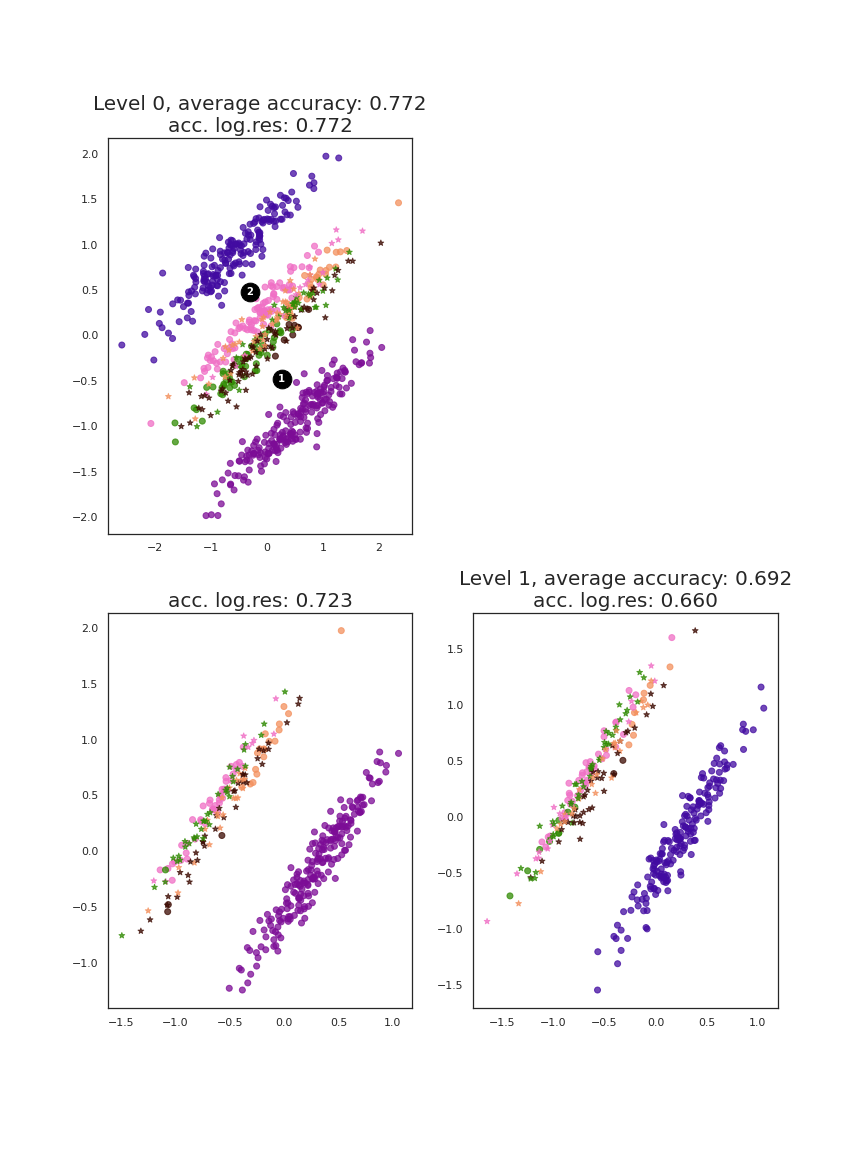
\includegraphics[width=.6\linewidth]{figs/complex_250_nuts.png}
    \caption[HmPPPCAs model performed on the complex Splatter data-set with 250 genes using NUTS]{\small \textbf{HmPPPCAs model performed on the complex Splatter data-set with 250 genes using NUTS.} \small A maximum accuracy of $0.772$ was found at level $0$. Performance did not improve after the top-level PPCA. The clusters found within the top-level PPCA have been numbered. The colours indicate different cell types. Data-points that were predicted correctly by the logistic regression are plotted with dots, incorrect predictions are plotted with stars.}
    \label{fig:complex_250_nuts}
\end{figure}


\begin{figure}
    \centering
    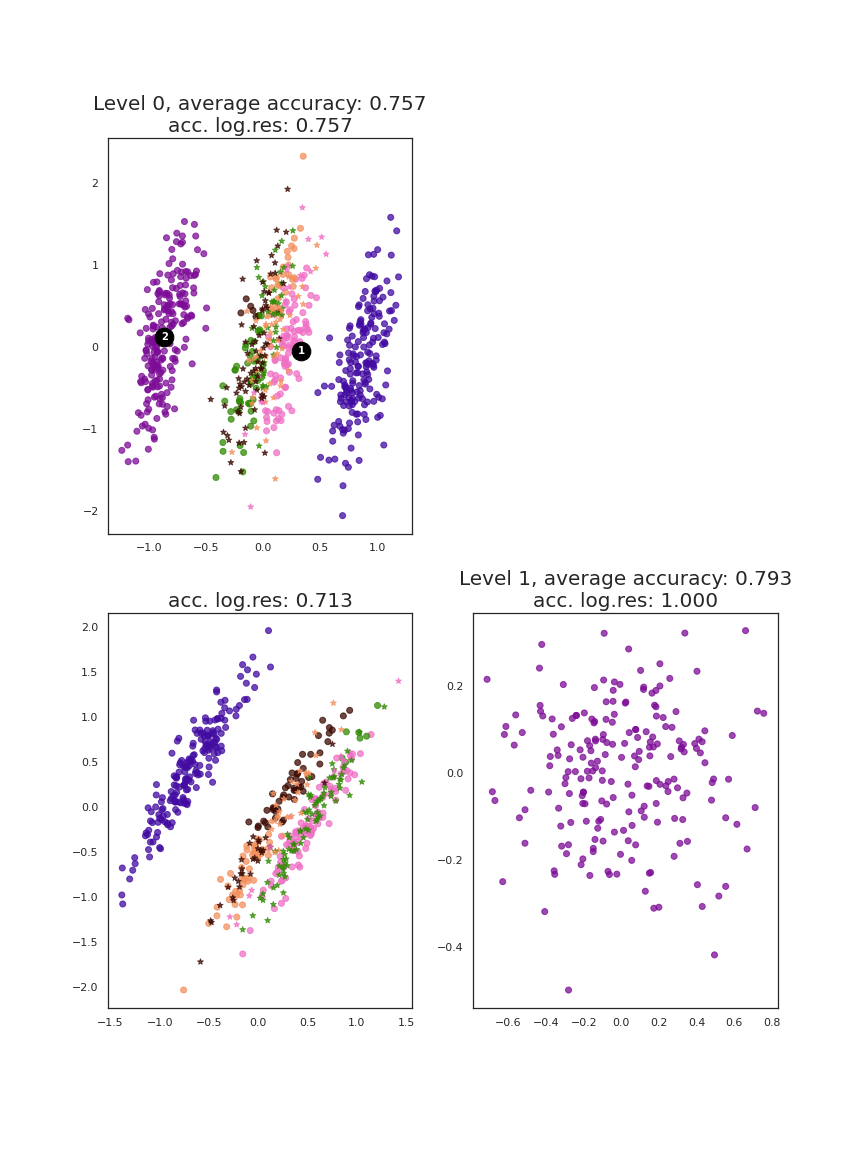
\includegraphics[width=.6\linewidth]{figs/complex_250_vb.png}
    \caption[HmPPPCAs model performed on the complex Splatter data-set with 250 genes using VB]{\small \textbf{HmPPPCAs model performed on the complex Splatter data-set with 250 genes using VB.} A maximum accuracy of $0.793$ was found after one level. The top-level PPCA achieved an accuracy of $0.757$. The clusters found within the top-level PPCA have been numbered. The colours indicate different cell types. Data-points that were predicted correctly by the logistic regression are plotted with dots, incorrect predictions are plotted with stars.}
    \label{fig:complex_250_vb}
\end{figure}


The UMAP and t-SNE baselines also achieved perfect accuracies of $1.0$ on the simple splatter data-sets. Slightly lower accuracies were achieved on the complex Splatter data-sets of low dimensionality, but this accuracy rose back to $1.0$ for the complex Splatter data-sets that contained at least $150$ genes. UMAP and t-SNE performed almost exactly equally good on the 5 genes complex data-sets, with t-SNE outperforming UMAP barely by a negligible difference. UMAP scores slightly higher on the 25 genes complex data-set and t-SNE on the 50 genes complex data-set. Together UMAP and t-SNE achieved the highest accuracy scores on the Splatter data-sets. The resulting visualizations of UMAP and t-SNE are given in Appendix \ref{sec:baselineresults}.

The result when using UMAP on the Darmanis data-set is given in Figure \ref{fig:darmanis_umap}, and the t-SNE result is given in Figure \ref{fig:darmanis_tsne}. Both of these methods outperformed the HmPPCAs. UMAP achieved the highest accuracy for the Nestorowa data-set, of which the results are visualized in Figure \ref{fig:nestorowa_nuts} (NUTS) and Figure \ref{fig:nestorowa_vb} (VB). In this case, however, t-SNE performed only slightly better than the two HmPPCAs models, and the UMAP accuracy was not much higher than the others.


% \textbf{Splatter data-sets}\\
% Figure \ref{fig:res_splatter} depicts the accuracies achieved on all splatter data-sets by the hmPPCA and the UMAP baseline. \todo{write more}

% \begin{figure}
%     \centering
%     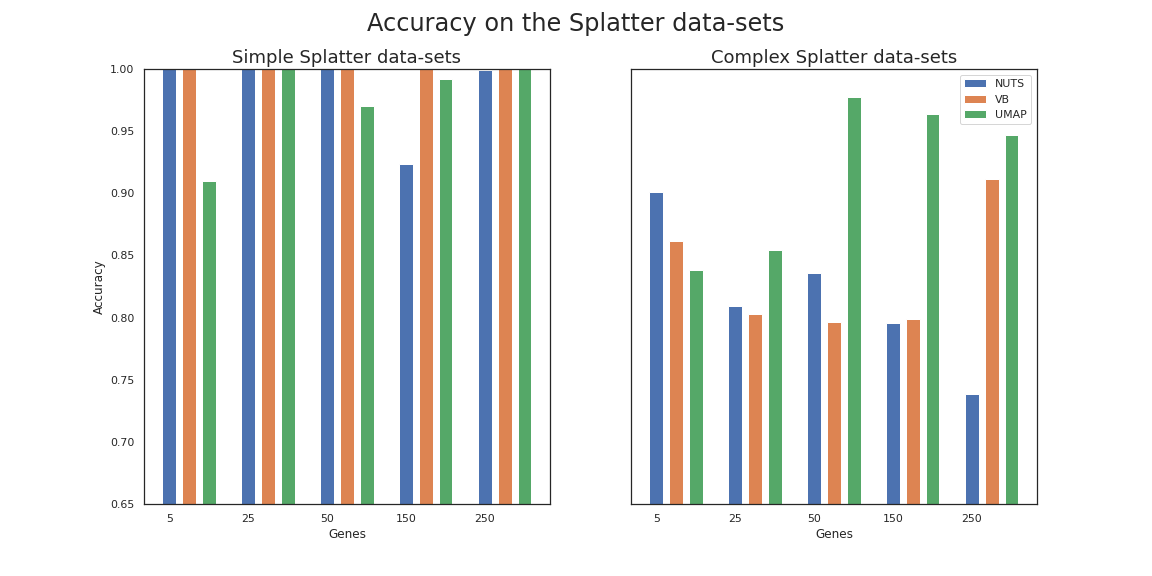
\includegraphics[width=\linewidth]{figs/Splatter_Accuracy_all.png}
%     \caption{\textbf{Accuracy on the simple (left) and complex (right) Splatter data-sets for all methods.} Accuracy is given on the y-axis and the number of genes in the data-set on the x-axis. Accuracy was measured after performing a logistic regression with a 5-fold cross validation. The results obtained through the hmPPCA are given in blue (when using NUTS) and orange (when using VB), the results of UMAP are plotted in green.}
%     \label{fig:res_splatter}
% \end{figure}
% \todo{needs to be updated, complex250 set is incorrect}

% \textbf{Damanis data-set}\\

\begin{figure}
    \centering
    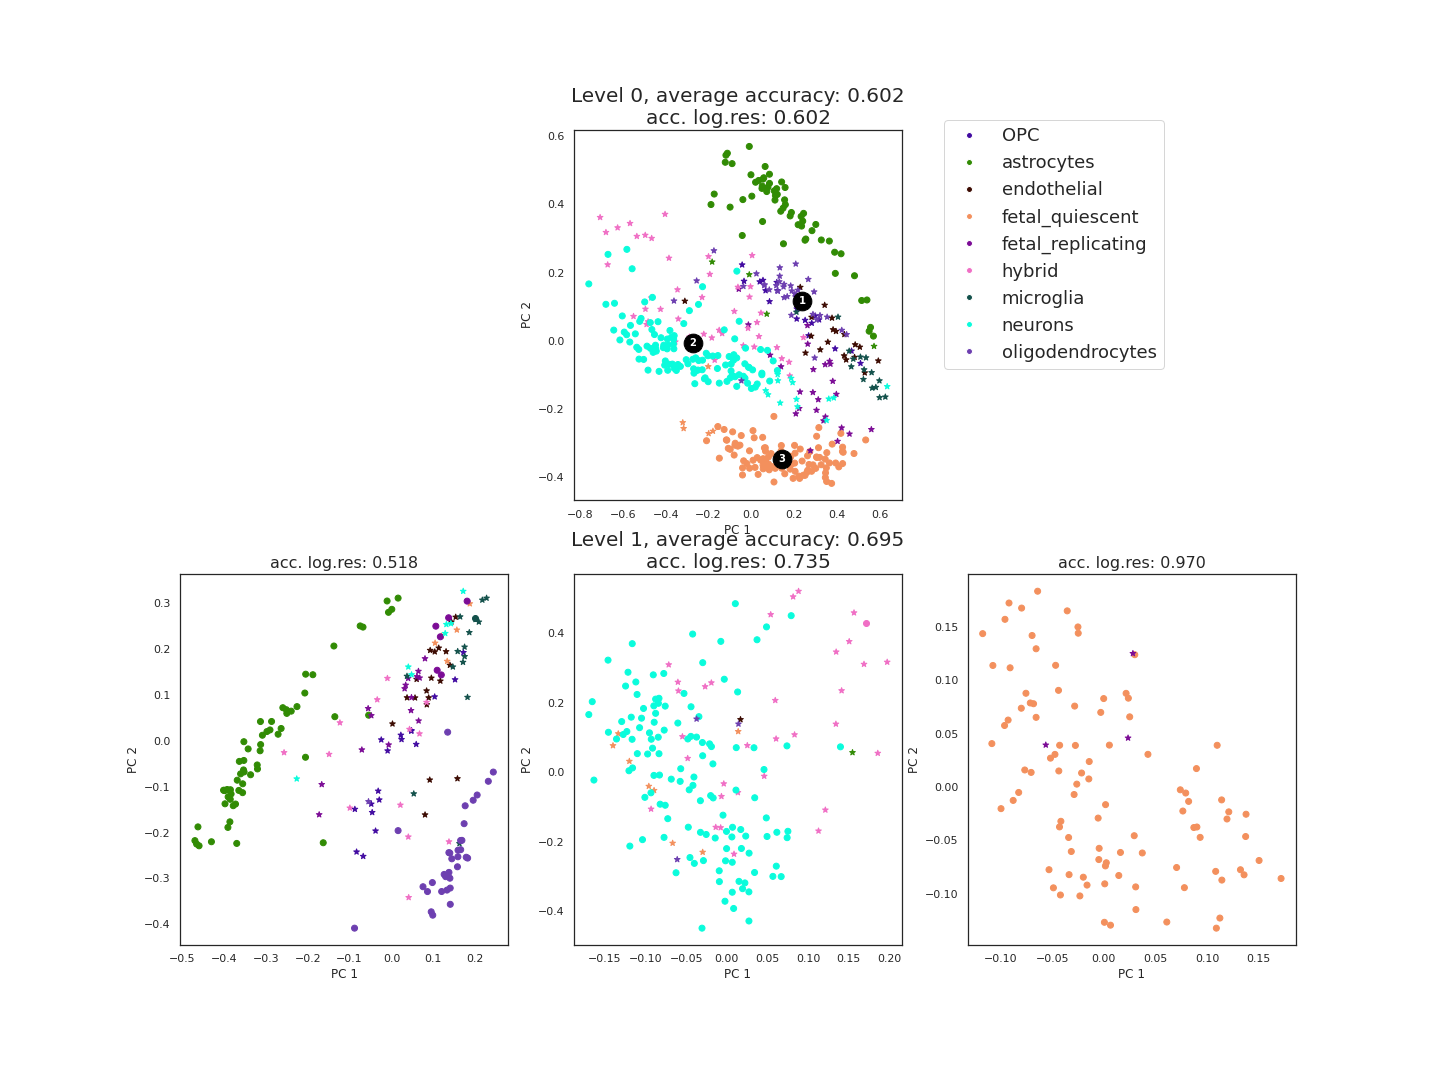
\includegraphics[width=\linewidth]{figs/Darmanis_tree_NUTS.png}
    \caption[The hmPPCAs analysis on the Darmanis data-set.]{\small \textbf{The hmPPCAs analysis on the Darmanis data-set.} \small NUTS was used for inference and one level was found. A maximum accuracy of $0.695$ was found at level $1$. The top-level PPCA achieved an accuracy of $0.602$. The clusters found within the top-level PPCA have been numbered. The colours indicate different cell types. Data-points that were predicted correctly by the logistic regression are plotted with dots, incorrect predictions are plotted with stars.}
    \label{fig:damanis_nuts}
\end{figure}

\begin{figure}
    \centering
    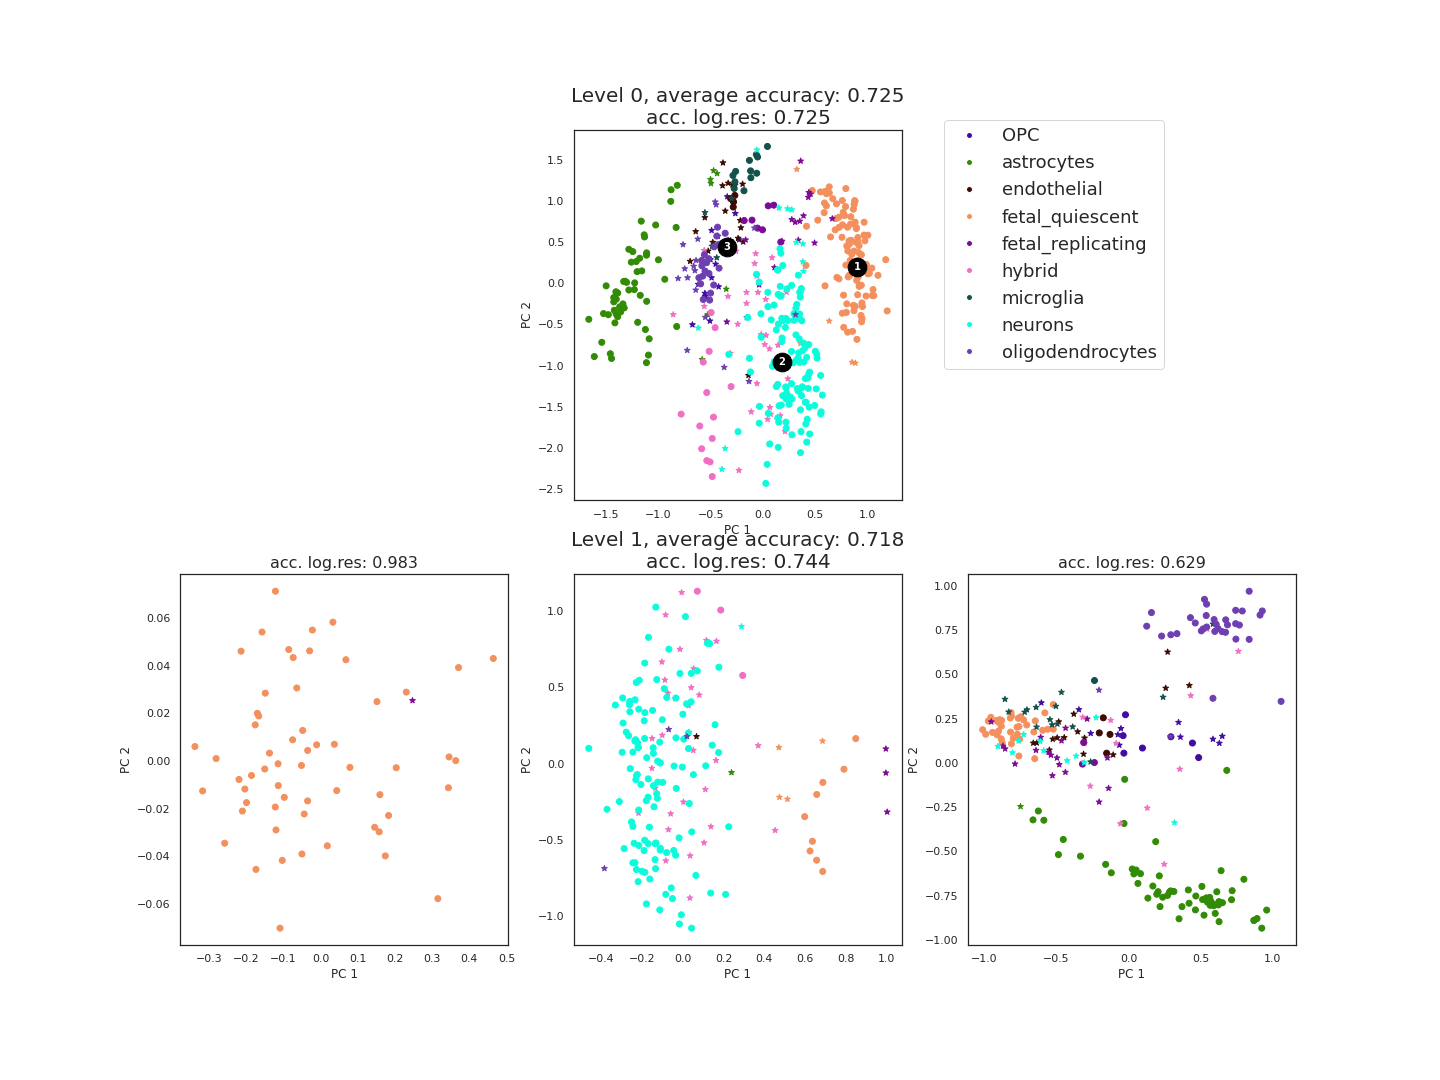
\includegraphics[width=\linewidth]{figs/Darmanis_tree_VB.png}
    \caption[The hmPPCAs analysis on the Darmanis data-set.]{\small \textbf{The hmPPCAs analysis on the Darmanis data-set.} \small VB was used for inference and one level was found. A maximum accuracy of $0.725$ was found at the top-level. The clusters found within the top-level PPCA have been numbered. The colours indicate different cell types. Data-points that were predicted correctly by the logistic regression are plotted with dots, incorrect predictions are plotted with stars.}
    \label{fig:darmanis_vb}
\end{figure}



% \textbf{Nestorowa data-set}\\

\begin{figure}
    \centering
    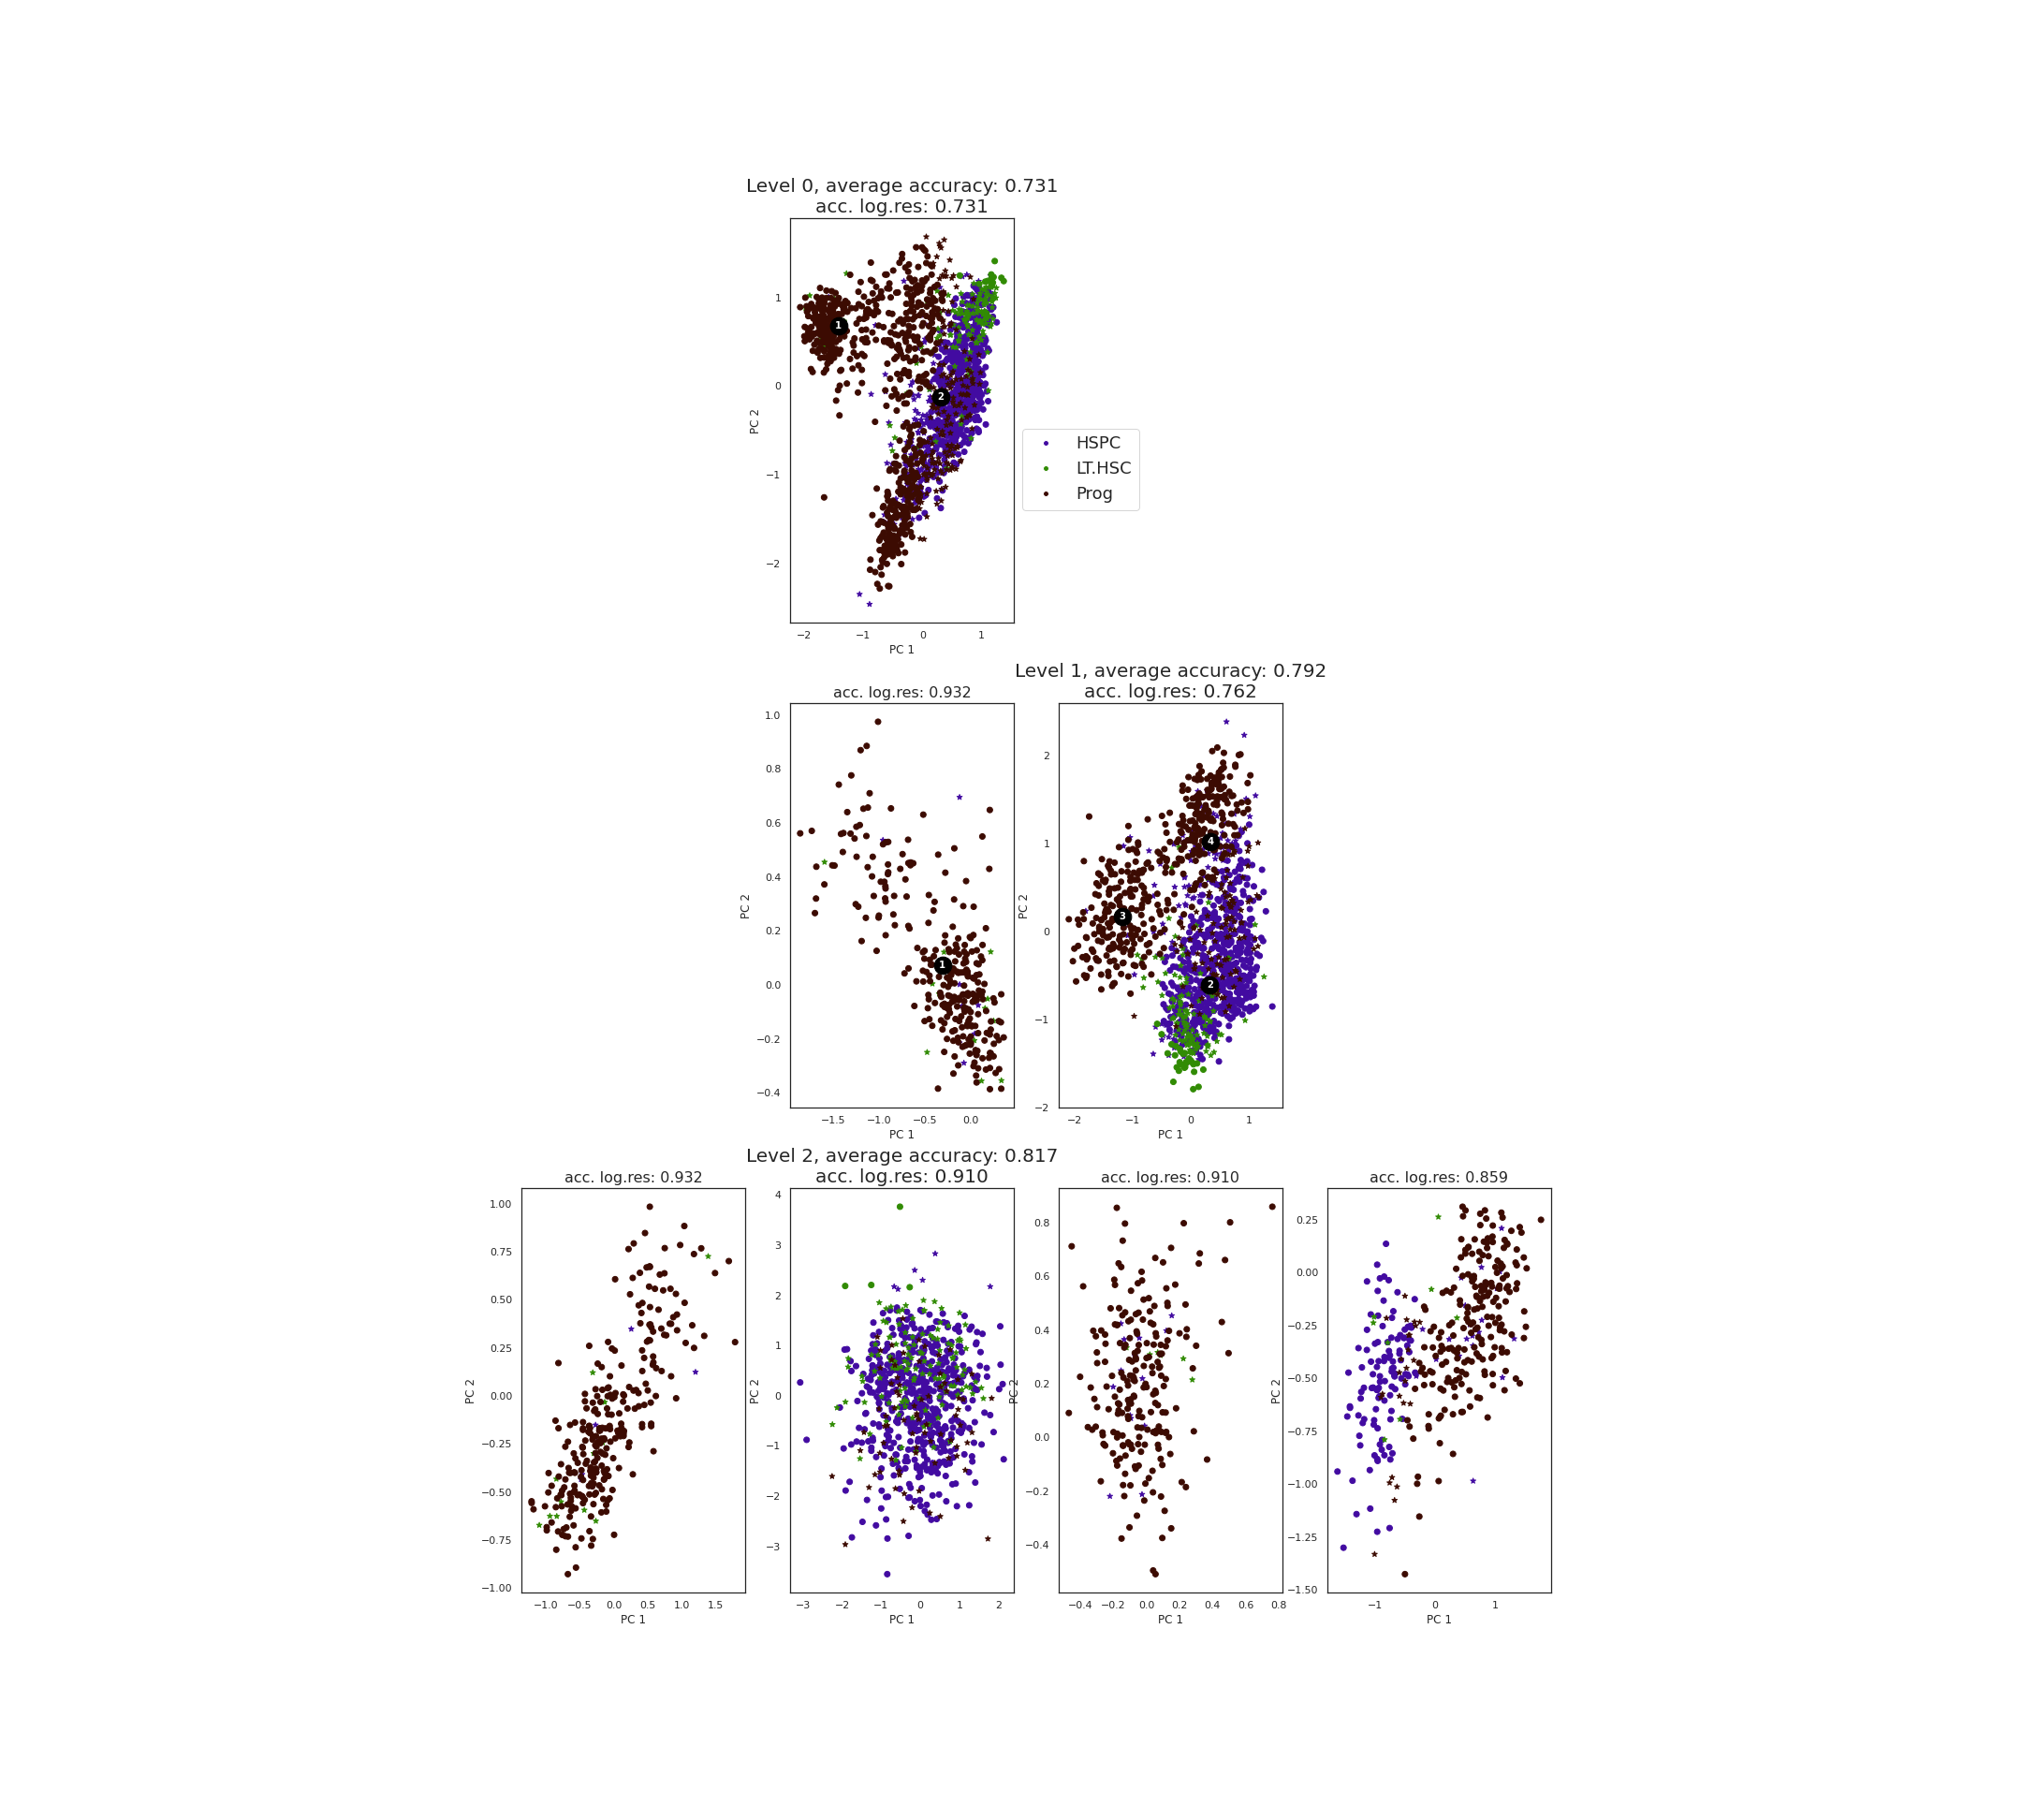
\includegraphics[width=0.95\linewidth]{figs/Nestorowa_tree_NUTS.png}
    \caption[The hmPPCAs analysis on the Nestorowa data-set.]{\small \textbf{The HmPPCAs analysis on the Nestorowa data-set.} \small NUTS was used as a sampling-method and five levels were found. A maximum accuracy of $0.817$ was found at level $2$. The top-level PPCA achieved an accuracy of $0.731$. The clusters found on each level have been numbered. The colours indicate different cell types. Data-points that were predicted correctly by the logistic regression are plotted with dots, incorrect predictions are plotted with stars.}
    \label{fig:nestorowa_nuts}
\end{figure}

\begin{figure}
    \centering
    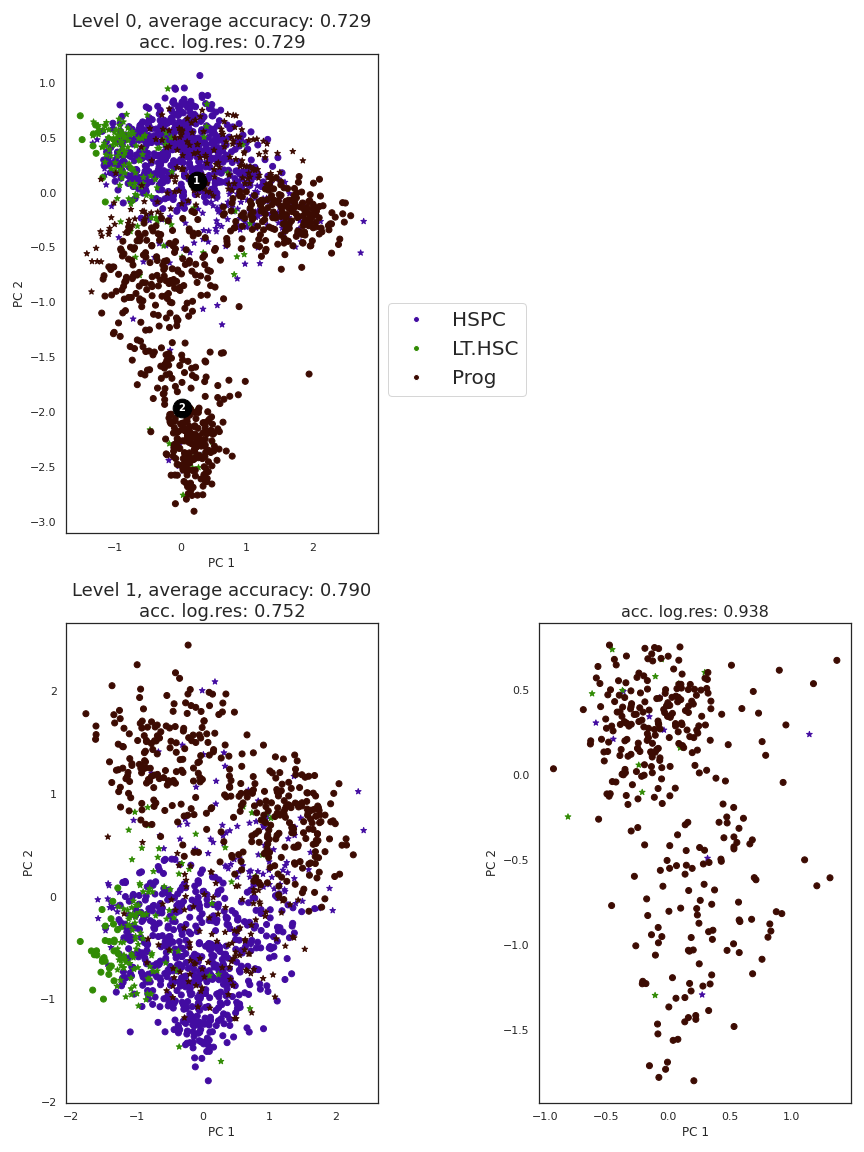
\includegraphics[width=.7\linewidth]{figs/Nestorowa_tree_VB.png}
    \caption[The hmPPCAs analysis on the Nestorowa data-set.]{\small \textbf{The HmPPCAs analysis on the Nestorowa data-set.} \small VB was used as a sampling-method and two levels were found. A maximum accuracy of $0.790$ was found at level $1$. The top-level PPCA achieved an accuracy of $0.729$. The clusters found within the top-level PPCA have been numbered. The colours indicate different cell types. Data-points that were predicted correctly by the logistic regression are plotted with dots, incorrect predictions are plotted with stars.}
    \label{fig:nestorowa_vb}
\end{figure}



\section{Computational cost}
Table \ref{tab:timetable} contains the computation times it took to infer the PPCA and MoPPCAs models on the Splatter data-sets. Each PPCA model was run only once at the top-level and its computation time is given. The MoPPCAs models were run repeatedly throughout the HmPPCAs models, so the average computation time of all MoPPCAs within the HmPPCAs is given instead. As expected, the PPCA models take less time to compute than the MoPPCAs models. This is the case for both NUTS and VB. We also see that VB takes considerably less time to infer solutions than NUTS for both the PPCA and the HmPPCAs models. The computational time goes up as the number of genes in the data-set rises, but more so when using NUTS than when using VB.

The time in seconds of the MoPPCAs models was also compared while taking the number of mixture components that the MoPPCAs models included into account. This was done for the Splatter data-sets and the results of this are shown in Figure \ref{fig:time_comps}. In some cases, a MoPPCAs model was initialized with a specific number of mixture components but ended up finding fewer mixture components. For this reason, both the number of initial mixture components and the number of found mixture components were taken into account separately. In both cases, there was no apparent relationship between the number of mixture components in a MoPPCAs model and the time it took to fit the model. Whereas sometimes the measured time became shorter when fewer mixture components were involved, this was the opposite for other cases, and in many cases, there was no effect to be observed at all.


\begin{table}
\setlength{\tabcolsep}{3pt}
    \caption[Computation times of PPCA and MoPPCAs models.]{\textbf{Computation times of PPCA and MoPPCAs models. In case multiple MoPPCAs were performed on a data-set within a HmPPCAs analyses, the average computation time of all MoPPCAs is reported.}}
    \centering
    \small
    \begin{tabular}{l|rrrrr|rrrrr}
          & \multicolumn{5}{r}{Splatter simple} & \multicolumn{5}{r}{Splatter complex}\\
          genes & 5 & 25 & 50 & 150 & 250 & 5 & 25 & 50 & 150 & 250\\
          \hline
        \makecell{PPCA\\(NUTS)} & 21.1 & 38.7 & 53.6 & 163.3 & 227.4 & 54.8 & 157.0 & 150.1 & 312.5 & 441.7\\
        \makecell{MoPPCAs\\(NUTS)} & 589.7 &  1313.2 & 1599.9 & 9266.6 & 10327.2 & 997.7 & 1945.1 & 2083.9 & 8409.1 & 17229.8\\
        \makecell{PPCA\\(VB)} & 2.8 & 4.4 & 5.3 & 11.3 & 14.0 & 7.0 & 16.1 & 11.3 & 20.8 & 14.3\\
        \makecell{MoPPCAs\\(VB)} & 31.5 & 48.6 & 101.1 & 276.6 & 208.3 & 11.5 & 28.3 & 48.7 & 210.7 & 104.9\\
    \end{tabular}
    % \medskip
    % \small
    % The average times in seconds to infer PPCA and MoPPCAs models when using NUTS and VB for all Splatter data-sets. NUTS takes more time to find a good fit of a model than ADVI. The computation time goes up when more genes are included into the set, but more so for NUTS than for ADVI.
    \label{tab:timetable}
\end{table}

\begin{figure}
    \centering
    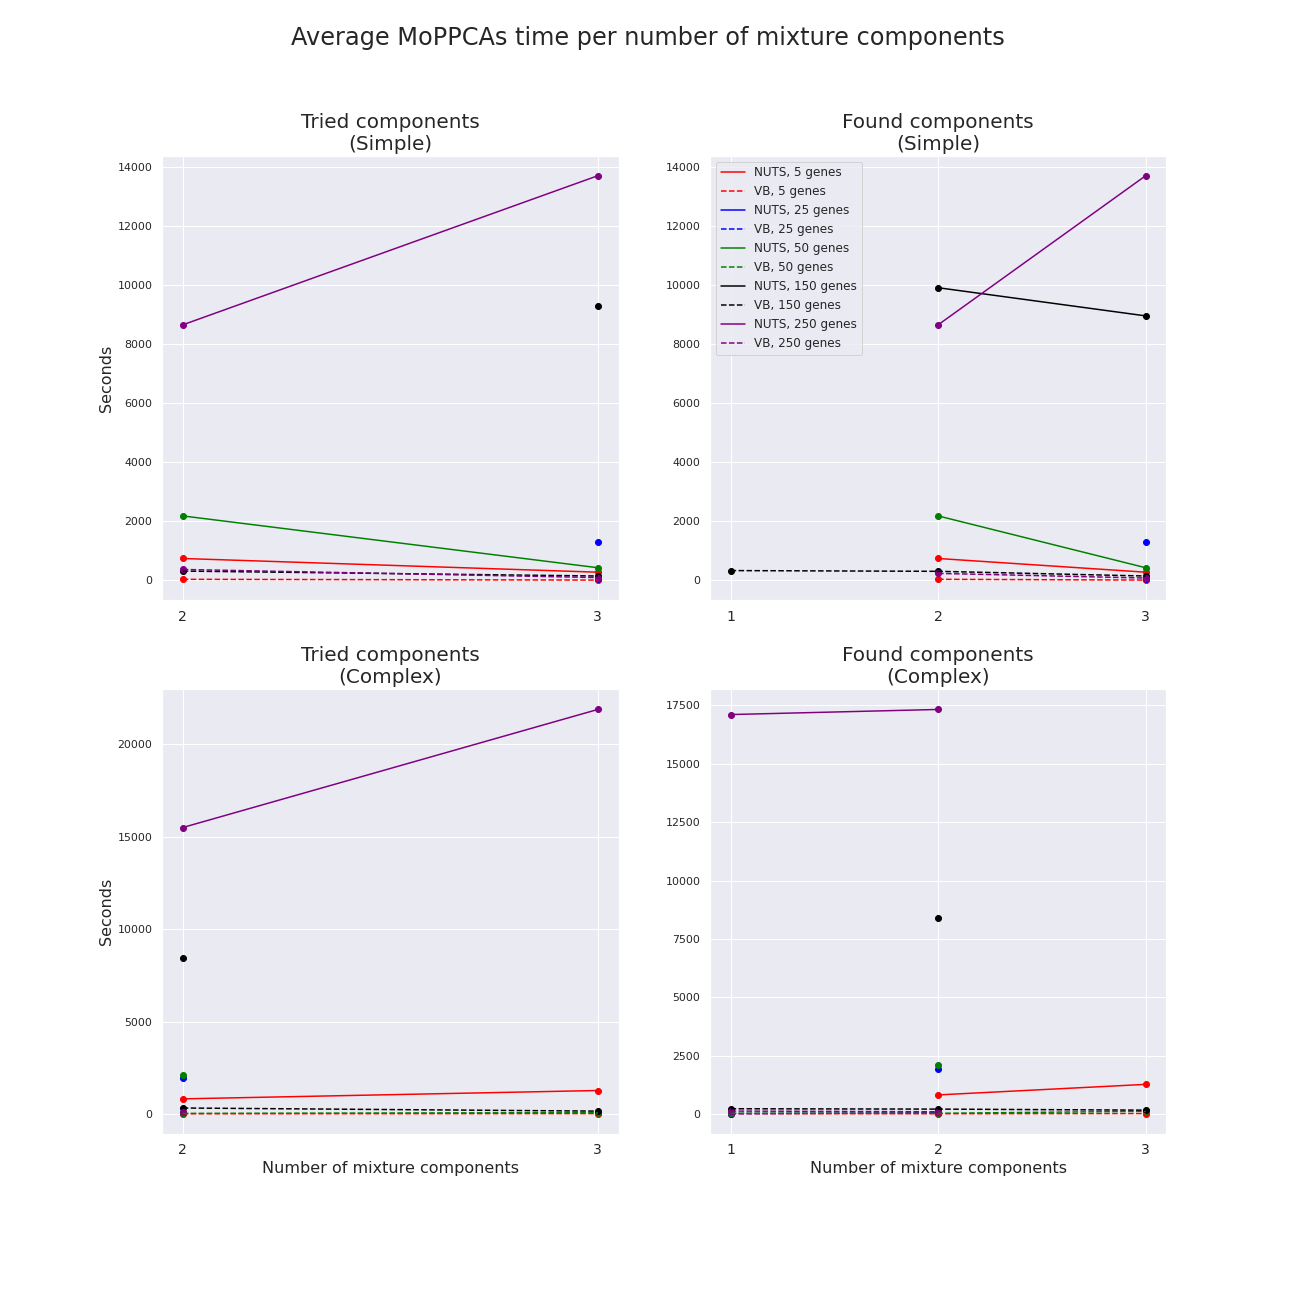
\includegraphics[width=\linewidth]{figs/time_mixture_comps.png}
    \caption[Average time to reach solution of MoPPCAs models in relation to their number of mixture components.]{\textbf{Average time to reach solution of MoPPCAs models in relation to their number of mixture components.}The two figures on the left show the (average) time is took for a MoPPCAs to be solved in relation to the number of mixture components that the model was suggested to find. The MoPPCAs models were always looking for either $2$ or $3$ mixture components. In some cases, less mixture components were found. The plots on the right relate the time to the number of mixture components that were found by the model, which may in some cases have been only $1$. The top two figures show this relation for the simple Splatter data-sets, the bottom two figures show this for the complex Splatter data-sets. In case of a dot that is not connected to another dot, no MoPPCAs model with a comparable number of mixture components has taken place in the HmPPCAs.}
    \label{fig:time_comps}
\end{figure}


% \subsection{Comparison NUTS and VB}

% \subsection{Our model in relation to other models}

% \section{Summary of all results}
